\let\negmedspace\undefined
\let\negthickspace\undefined
\documentclass[journal]{IEEEtran}
\usepackage[a5paper, margin=10mm, onecolumn]{geometry}
%\usepackage{lmodern} % Ensure lmodern is loaded for pdflatex
\usepackage{tfrupee} % Include tfrupee package

\setlength{\headheight}{1cm} % Set the height of the header box
\setlength{\headsep}{0mm}     % Set the distance between the header box and the top of the text

\usepackage{gvv-book}
\usepackage{gvv}
\usepackage{cite}
\usepackage{amsmath,amssymb,amsfonts,amsthm}
\usepackage{algorithmic}
\usepackage{graphicx}
\usepackage{textcomp}
\usepackage{xcolor}
\usepackage{txfonts}
\usepackage{listings}
\usepackage{enumitem}
\usepackage{mathtools}
\usepackage{gensymb}
\usepackage{comment}
\usepackage[breaklinks=true]{hyperref}
\usepackage{tkz-euclide} 
\usepackage{listings}
% \usepackage{gvv}                                        
\def\inputGnumericTable{}                                 
\usepackage[latin1]{inputenc}                                
\usepackage{color}                                            
\usepackage{array}                                            
\usepackage{longtable}                                       
\usepackage{calc}                                             
\usepackage{multirow}                                         
\usepackage{hhline}                                           
\usepackage{ifthen}                                           
\usepackage{lscape}
\usepackage{circuitikz}
\tikzstyle{block} = [rectangle, draw, fill=blue!20, 
    text width=4em, text centered, rounded corners, minimum height=3em]
\tikzstyle{sum} = [draw, fill=blue!10, circle, minimum size=1cm, node distance=1.5cm]
\tikzstyle{input} = [coordinate]
\tikzstyle{output} = [coordinate]


\begin{document}

\bibliographystyle{IEEEtran}
\vspace{3cm}

\title{12.6.5.3.2}
\author{EE24BTECH11064 - Harshil Rathan}
 \maketitle
% \newpage
% \bigskip
{\let\newpage\relax\maketitle}

\renewcommand{\thefigure}{\theenumi}
\renewcommand{\thetable}{\theenumi}
\setlength{\intextsep}{10pt} % Space between text and floats


\numberwithin{equation}{enumi}
\numberwithin{figure}{enumi}
\renewcommand{\thetable}{\theenumi}

\textbf{Question}:\\
Find the local maxima and local minima, if any of the following functions. Find also the local maximum and local minimum values, as the case may be 
\begin{align*}
    g(x) = x^3-3x
\end{align*}\\ 
\solution \\
\textbf{Theory} \\
The first derivative, $g'(x)$ gives us the critical points (where the slope is zero or undefined) 
\begin{align}
     g'(x) = 3x^2- 3
     \label{0.1}
\end{align}
Set derivative equal to 0 
\begin{align}
    g'(x) = 3x^2-3 = 0 
\end{align}
\begin{align}
    x = \pm 1 
\end{align}
The critical points are 1 and -1 \\
The second derivative $g''(x)$ helps us determine the nature of critical points 
\begin{align}
  g''(x) = 6x
\end{align}
At $x = 1$ 
\begin{align}
    g''(1) = 6 > 0 
\end{align}
indicating a local minimum \\
For $x = -1$ 
\begin{align}
    g''(-1) = -6 < 0
\end{align}
indicating a local maximum \\
Calculating local maxima and minimum values \\
At $x=1$
\begin{align}
   g(1) = 1 - 3 = - 2 
\end{align}
Local minimum value is -2 \\
At $x=-1$
\begin{align}
  g(-1) = (-1)^3 -3(-1) = 2 
\end{align}
Local maximum value is 2  \\
Local maximum : At \(x = -1\), the maximum value is \(g(-1) = 2\). \\
Local minimum : At \(x = 1\), the minimum value is \(g(1) = -2\).

\textbf{Computational Solution Using Gradient Descent and Ascent}\\
To verify the analytical results, we use gradient descent and gradient ascent to find the local minimum and maximum, respectively.\\
Gradient Descent for local minimum : \\ 
 - Start with $x_0 = 0.5$ (close to 1.0)\\
 - Update $x$ iteratively using 
\begin{align}
    x_{1} = x_0 - \eta \cdot g'(x_0)
\end{align}
where :
\begin{align}
    \eta = 0.1 
\end{align}
\begin{align}
    g'(x) = 3x^2 - 3 
\end{align}
\begin{align}
    x_{n+1} = x_n - \eta \cdot (3x_n^2 -3)
\end{align}
Stop the iteration when the change in x is smaller than a specified tolerance $(10^{-6})$\\
Gradient Ascent for local maxima \\
- Start with $x_0 = - 1.5$ (close to -1)\\
- Update x iteratively 
\begin{align}
  x_1 = x_0 + \eta \cdot g'(x_0)
\end{align}
\begin{align}
    x_{n+1} = x_n + \eta\cdot(3x_n^2-3)
\end{align}
\textbf{Computational Results} \\
 - Local minimum 
 \begin{align}
     x \approx 1.000,\text{ } g(x) \approx -2.000
 \end{align} 
- Local maximum
\begin{align}
    x \approx -1.000 , \text{ }g(x)  \approx 2.000
\end{align}
\begin{figure}
    \centering
    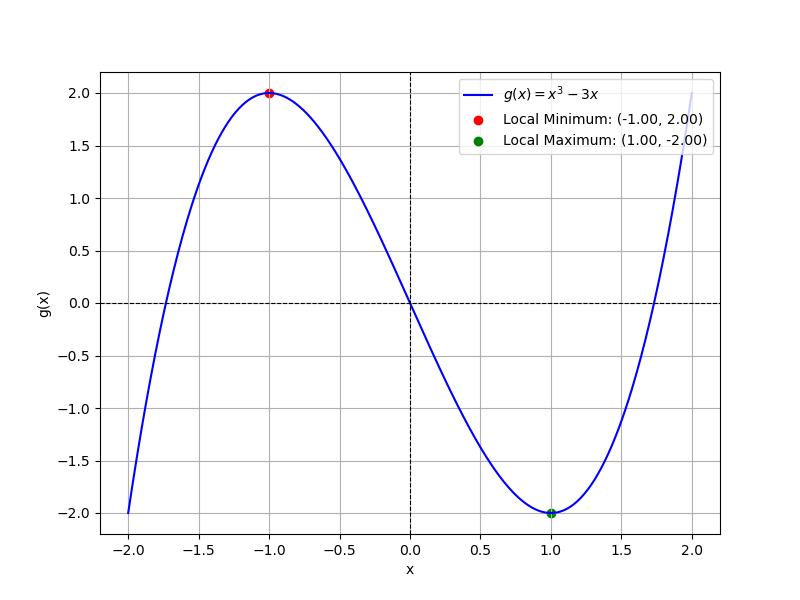
\includegraphics[width=\columnwidth]{figs/Figure_1.png}
\end{figure}
\end{document}



